\documentclass[10pt]{../usamts}

\realname{Juni Kim}
\username{junikimm}
\usamtsid{38002}
\usamtsyear{35}
\usamtsround{2}

\begin{document}

%%%%%%%%%%%%%%%%%%%%%%%%%%%%%%%%%%%%%
%%%%%%%%%%                 %%%%%%%%%%
%%%%%%%%%%    Problem 1    %%%%%%%%%%
%%%%%%%%%%                 %%%%%%%%%%
%%%%%%%%%%%%%%%%%%%%%%%%%%%%%%%%%%%%%
\begin{solution}
\begin{center}
\begin{asy}
unitsize(4cm);
defaultpen(fontsize(30pt));
real HRT3 = sqrt(3) / 2;

void drawCircle(real x, real y, real r) {
path p = circle((x,y), r);
draw(p);
fill(p, white);
}

void drawCell(int gx, int gy, int num) {
real x = 0.5 * gx;
real y = HRT3 * gy;
drawCircle(x, y, 0.35);
label((string)num, (x,y));
}

void drawNumber(int gx, int gy, int number) {
real x = 0.5 * gx;
real y = HRT3 * gy;
label(scale(1.5)*string(number), (x, y));
}

void drawEdge(int gx1, int gy1, int gx2, int gy2, bool doubled) {
real x1 = 0.5 * gx1;
real y1 = HRT3 * gy1;
real x2 = 0.5 * gx2;
real y2 = HRT3 * gy2;
if (doubled) {
real dx = x2 - x1;
real dy = y2 - y1;
real ox = -0.035 * dy / sqrt(dx * dx + dy * dy);
real oy = 0.035 * dx / sqrt(dx * dx + dy * dy);
draw((x1+ox,y1+oy)--(x2+ox,y2+oy));
draw((x1-ox,y1-oy)--(x2-ox,y2-oy));
} else {
draw((x1,y1)--(x2,y2));
}
}

drawEdge(2, 0, 4, 0, true);
drawEdge(2, 0, 1, 1, true);
drawEdge(2, 0, 3, 1, true);
drawEdge(4, 0, 3, 1, false);
drawEdge(4, 0, 5, 1, false);
drawEdge(1, 1, 0, 2, false);
drawEdge(1, 1, 2, 2, false);
drawEdge(1, 1, 3, 1, false);
drawEdge(3, 1, 2, 2, true);
drawEdge(3, 1, 4, 2, true);
drawEdge(3, 1, 5, 1, false);
drawEdge(5, 1, 4, 2, true);
drawEdge(5, 1, 6, 2, false);
drawEdge(0, 2, 1, 3, false);
drawEdge(0, 2, 2, 2, false);
drawEdge(2, 2, 1, 3, false);
drawEdge(2, 2, 3, 3, true);
drawEdge(2, 2, 4, 2, false);
drawEdge(4, 2, 3, 3, false);
drawEdge(4, 2, 5, 3, false);
drawEdge(4, 2, 6, 2, false);
drawEdge(6, 2, 5, 3, true);
drawEdge(1, 3, 3, 3, true);
drawEdge(3, 3, 5, 3, false);

int[][] numbers = {
{28, 22, 27},
{23, 33, 35, 24},
{10, 21, 25},
{30, 32}};

drawCell(2, 0, numbers[3][0]);
drawCell(4, 0, numbers[3][1]);
drawCell(1, 1, numbers[2][0]);
drawCell(3, 1, numbers[2][1]);
drawCell(5, 1, numbers[2][2]);
drawCell(0, 2, numbers[1][0]);
drawCell(2, 2, numbers[1][1]);
drawCell(4, 2, numbers[1][2]);
drawCell(6, 2, numbers[1][3]);
drawCell(1, 3, numbers[0][0]);
drawCell(3, 3, numbers[0][1]);
drawCell(5, 3, numbers[0][2]);
\end{asy}
\end{center}
\end{solution}

%%%%%%%%%%%%%%%%%%%%%%%%%%%%%%%%%%%%%
%%%%%%%%%%                 %%%%%%%%%%
%%%%%%%%%%    Problem 2    %%%%%%%%%%
%%%%%%%%%%                 %%%%%%%%%%
%%%%%%%%%%%%%%%%%%%%%%%%%%%%%%%%%%%%%

\begin{solution}
We will just approach this by bashing. Let $a_n$ denote the number of six-digit codes possible when $n$ of the digits on the board have been smudged.
For our base case, $a_1 = 1$ because the only possible code is having all the digits be the same.

\begin{claim}
    For $2 \le n \le 6$,
    $$a_n = n^6 - \sum_{k=1}^{n-1} \binom{n}{k} a_k$$
\end{claim}
\begin{proof}
    The reasoning is fairly straightforward. The number of combinations where we use at most $n$ of our allotted digits is $n^6$. Now, we just need to remove the cases where we're not using all $n$ digits. There are $\binom{n}{k} a_k$ ways in which we can first choose a subset of $k$ digits and then make a string using all $k$ digits at least once.
\end{proof}
\begin{align*}
a_2 &= 2^6 - \binom{2}{1} \cdot a_1 = 62\\
a_3 &= 3^6 - \binom{3}{2} \cdot a_2 - \binom{3}{1} \cdot a_1 = 540\\
a_4 &= 4^6 - \binom{4}{3} \cdot a_3 - \binom{4}{2} \cdot a_2 - \binom{4}{1} \cdot a_1 = 1560\\
a_5 &= 5^6 - \binom{5}{4} \cdot a_4 - \binom{5}{3} \cdot a_3 - \binom{5}{2} \cdot a_2 - \binom{5}{1} \cdot a_1 = 1800\\
a_6 &= 6^6 - \binom{6}{5} \cdot a_5 - \binom{6}{4} \cdot a_4 - \binom{6}{3} \cdot a_3 - \binom{6}{2} \cdot a_2 - \binom{6}{1} \cdot a_1 = 720\\
\end{align*}

It is clear from these calculations that we get the most possible combinations when 5 of the digits have been smudged.

\end{solution}


%%%%%%%%%%%%%%%%%%%%%%%%%%%%%%%%%%%%%
%%%%%%%%%%                 %%%%%%%%%%
%%%%%%%%%%    Problem 3    %%%%%%%%%%
%%%%%%%%%%                 %%%%%%%%%%
%%%%%%%%%%%%%%%%%%%%%%%%%%%%%%%%%%%%%
\begin{solution}
Note that a set of three numbers is \textit{balanced} if and only if their sum is congruent to 0 mod 3.

We establish a coordinate system before proceeding. The rows will be 0-indexed from bottom to top. So, the top row will be row 9, while the bottom row will be row 0. We will also 0-index each hexagon on each row going from left to right. So, $a_{i,j}$ is the $j+1$th hexagon on the $i+1$th row from the bottom.

We start by independently filling in the bottom numbers such that they take the values $a_{0,0} \dots a_{0,9}$ going from left to right. We can freely choose each number because no three hexagons on the bottom row are mutually adjacent.

Now, we claim that the entire rest of the grid is determined by the bottom row. In particular, $$a_{i,j} \equiv (-1)^{i} \sum_{k=0}^{i} \binom{i}{k} a_{0,j+k} \mod 3$$

This is easy to see by induction. The base case, for row 0, is trivial. For the inductive step, the \textit{balanced} condition implies that
\begin{align*}
    a_{i,j} &\equiv -\paren{a_{i-1,j}+a_{i-1,j+1}} \mod 3\\
            &\equiv (-1)^{i} \paren{\sum_{k=0}^{i-1} \binom{i-1}{k} a_{0,j+k} + \sum_{k=0}^{i-1} \binom{i-1}{k} a_{0,j+1+k}} \mod 3\\
            &\equiv (-1)^{i}\paren{a_{0,j} + a_{0,i+j} + \sum_{k=0}^{i-2} \paren{\binom{i-1}{k} + \binom{i-1}{k+1}} a_{0,j+k+1} } \mod 3\\
            &\equiv (-1)^{i}\paren{a_{0,j} + a_{0,i+j} + \sum_{k=1}^{i-1} \binom{i}{k} a_{0,j+k} } \tag{hockey stick} \mod 3\\
            &\equiv (-1)^{i} \sum_{k=0}^{i} \binom{i}{k} a_{0,j+k} \mod 3\\
\end{align*}

We now proceed onto the final calculation. Note that
$$\binom{9}{0} = \binom{9}{9} = 1$$
$$\binom{9}{1} = \binom{9}{8} = 9, 3\,|\,9$$
$$\binom{9}{2} = \binom{9}{7} = 36, 3\,|\,36$$
$$\binom{9}{3} = \binom{9}{6} = 84, 3\,|\,84$$
$$\binom{9}{4} = \binom{9}{5} = 126, 3\,|\,126$$

So it is clear that
\begin{align*}
    a_{9,0} &\equiv -\paren{\sum_{k=0}^{9} \binom{9}{k} a_{0,k}} \mod 3\\
    &\equiv -\paren{a_{0,0} + a_{0,9}} \mod 3\\
\end{align*}

Since $a_{0,0} + a_{0,9} + a_{9,0} \equiv 0 \mod 3$, they are balanced.

\end{solution}


%%%%%%%%%%%%%%%%%%%%%%%%%%%%%%%%%%%%%
%%%%%%%%%%                 %%%%%%%%%%
%%%%%%%%%%    Problem 4    %%%%%%%%%%
%%%%%%%%%%                 %%%%%%%%%%
%%%%%%%%%%%%%%%%%%%%%%%%%%%%%%%%%%%%%
\begin{solution}
\begin{figure}
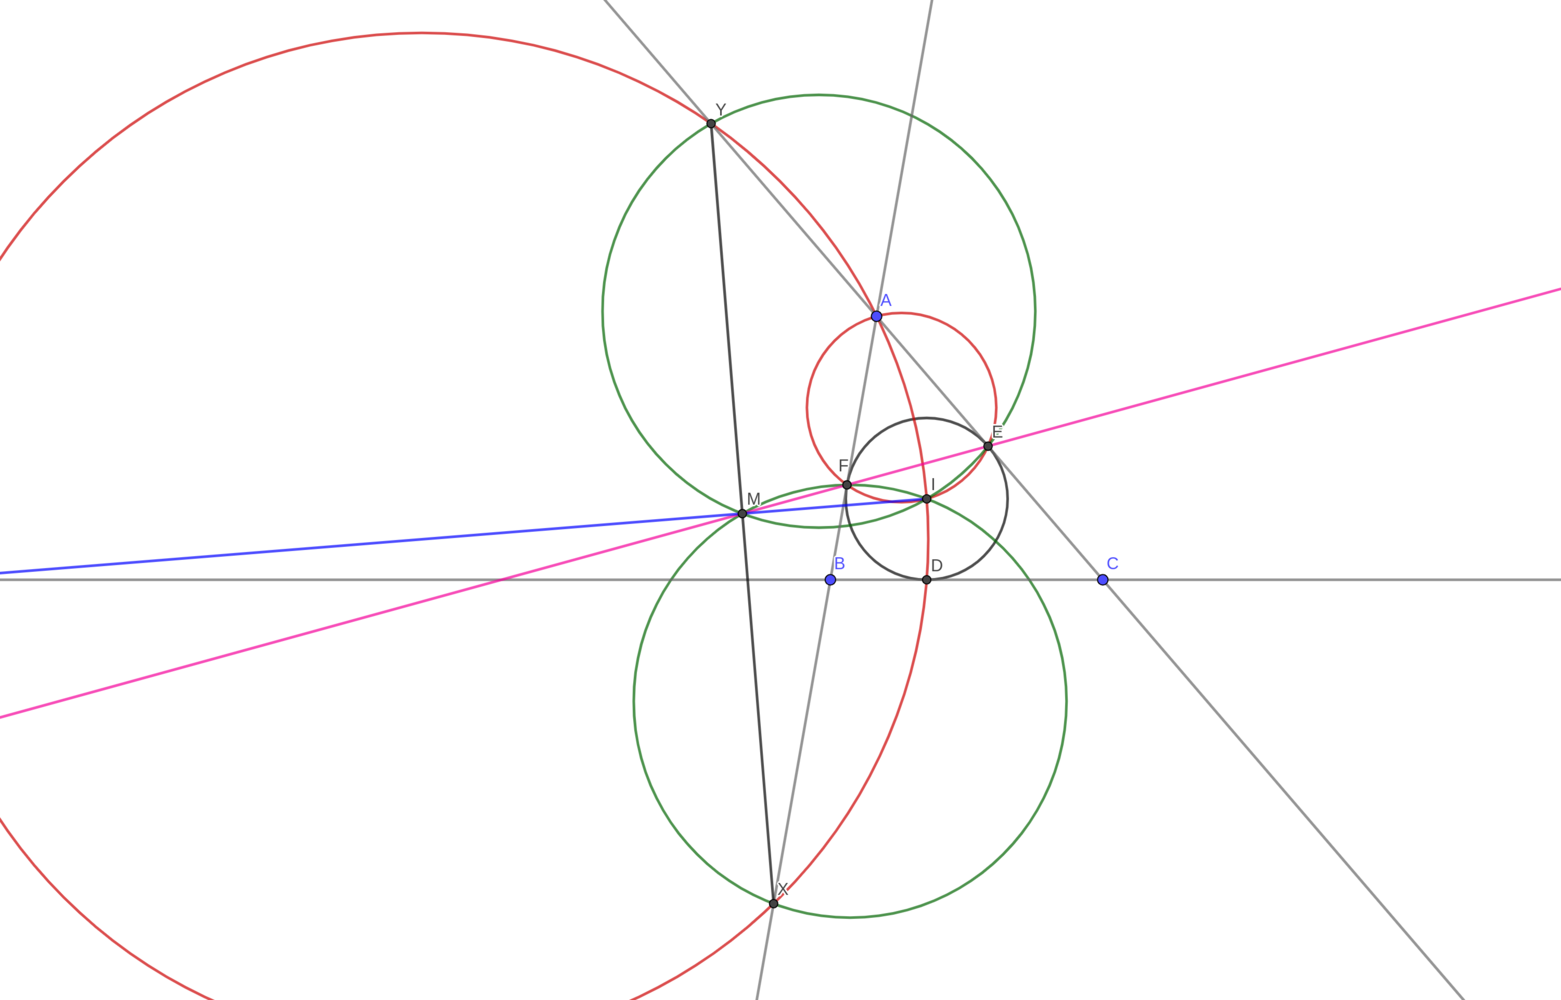
\includegraphics[width=12cm]{round2/p4diagram.png}
\caption{The Diagram}
\end{figure}

Note that $AFIE$ is a cyclic quadrilateral because $\angle IFA = \angle IEA = 90^\circ$. We therefore know that there is a spiral similarity that sends $\triangle FIE$ to $\triangle XIY$. Since $\triangle FIE$ is an isosceles triangle, so is $XIY$. Therefore, the midpoint of $XY$, which we denote $M$, is also the foot of the perpendicular from $I$ to $XY$. Since $\angle IEY = 90$ and $\angle IFX = 90^\circ$, It follows that $IEMY$ and $IFMX$ are cyclic quadrilaterals. Now, note that $\angle MFI = 180^\circ - \angle MXI = 180^\circ - \angle YXI = 180^\circ - \angle EFI$ by the spiral similarity from before. So, $M,E,F$ are collinear and we are done.
\end{solution}

%%%%%%%%%%%%%%%%%%%%%%%%%%%%%%%%%%%%%
%%%%%%%%%%                 %%%%%%%%%%
%%%%%%%%%%    Problem 5    %%%%%%%%%%
%%%%%%%%%%                 %%%%%%%%%%
%%%%%%%%%%%%%%%%%%%%%%%%%%%%%%%%%%%%%
\begin{solution}
This was quite a painful construction problem\dots

The answer is all $n,m$ such that \fbox{$n+m \equiv 1 \mod 4$ or $n \equiv m \mod 4$}.

\begin{claim}
    The above condition must hold.
\end{claim}
\begin{proof}
    Let $T$ contain $l$ points of the form $(x_i,y_i)$.
    $$\sum_i x_i + \sum_i y_i \equiv \sum_{k=1}^{m+n-1} 1 + \sum_{k=1}^{m+n-1} 1 \equiv 0 \mod 2$$
    $$\sum_i x_i + y_i \equiv \sum_{k=m+1}^{2m+n-1} 1 \equiv \frac{1}{2} \paren{m+n-1}\paren{3m+n} \mod 2$$
    Since $\paren{\sum_i x_i} + \paren{\sum_i y_i} = \sum_i \paren{x_i+y_i}$, $\frac{1}{2} (m+n-1)(3m+n)$ must be even to prevent a contradiction.
    So, it follows that $(m+n-1)(n-m)$ is congruent to 0 mod 4. Since $(n-m)$ and $(m+n-1)$ always differ in parity, it follows that exactly one of them must be divisible by 4. This implies that either $n+m \equiv 1 \mod 4$ or $n \equiv m \mod 4$.
\end{proof}

\newcommand{\mainaxis}{
    Select the points on the main axis so that each diagonal intersects exactly one point:
    \begin{enumerate}
        \item Select all the points of the form $(m, m+2k-1)$ for $1 \leq k \leq \floor{\frac{n}{2}}$
        \item Select all the points of the form $(m, m-2k)$ for $1 \leq k \leq \floor{\frac{m-1}{2}}$
        \item Select all the points of the form $(m+2k, m)$ for $1 \leq k \leq \floor{\frac{n-1}{2}}$
        \item Select all the points of the form $(m-2k+1, m)$ for $1 \leq k \leq \floor{\frac{m}{2}}$
    \end{enumerate}
}

In the next few pages, we will show that there always exists a construction for the subset $T$ if $n+m \equiv 1 \mod 4$ or $n \equiv m \mod 4$.

\clearpage
We first handle the case where $n \equiv m \mod 4$. Without loss of generality, assume that $n \geq m$. If $m \geq n$, we can just reflect our current construction across the point $(m,m)$ and translate it accordingly. We then apply the following steps:
\begin{enumerate}
    \item Select the point $(m,m)$ if and only if $m$ is odd.
    \item \mainaxis
    After this process is done, the lines $x+y = k$ where $m+1 \leq k < 2m$ and $2m < k \leq 2m+n-1$ will each intersect exactly one point from our set.
    \item Select points on the diagonal $x+y = 2m$ so that all the rows and columns in the ``center'' intersect an odd number of points:
    \begin{enumerate}
        \item Select all the points of the form $(m+2k-1,m-2k+1)$ for $1 \leq k \leq \floor{\frac{m}{2}}$
        \item Select all the points of the form $(m-2k,m+2k)$ for $1 \leq k \leq \floor{\frac{m-1}{2}}$
    \end{enumerate}
    After this process is done, the lines $x=m$, $y=m$, and $x+y = 2m$ will intersect $\floor{\frac{m-1}{2}} + \floor{\frac{n}{2}} + (m \mod 2)$, $\floor{\frac{n-1}{2}} + \floor{\frac{m}{2}} + (m \mod 2)$, and $\floor{\frac{m-1}{2}} + \floor{\frac{m}{2}} + (m \mod 2)$ points respectively. Since $m \equiv n \mod 4$, these expressions will all be odd. Furthermore, the lines $x=k$ for all $1 \leq k \leq 2m-1$ and $x=k$ for all $1 \leq k \leq 2m-1$ will all intersect exactly one point from our set.
    \item Create a ``tail'' to cover all of the outer rows and columns:
    \begin{enumerate}
        \item Select all the points of the form $\paren{ m+2\floor{\frac{m}{2}}-1+2k, m-2\floor{\frac{m}{2}}+2 }$ for $1 \leq k \leq \frac{n-m}{2}$. This adds an even number of points since $m \equiv n \mod 4$, so the line $y = m-2\floor{\frac{m}{2}}+2$ still intersects an odd number of points.
        \item Select all the points of the form $\paren{ m-2\floor{\frac{m-1}{2}}+1, m+2\floor{\frac{m-1}{2}}+2k }$ for $1 \leq k \leq \frac{n-m}{2}$. This adds an even number of points for the same reason as before, so the line $x = m-2\floor{\frac{m-1}{2}}+1$ still intersects an odd number of points.
    \end{enumerate}
    With the addition of these points, all horizontal and vertical lines now intersect an odd number of points; all lines of the form $x = k$ for all $2m \leq k < m+n$ and $y=k$ for all $2m \leq k < m+n$ will also intersect exactly one point.
    
    Let the set of points that we selected in Step 4 be denoted $U$. Notice that $\paren{ m+2\floor{\frac{m}{2}}-1+2k}+\paren{m-2\floor{\frac{m}{2}}+2} = \paren{m-2\floor{\frac{m-1}{2}}+1}+\paren{m+2\floor{\frac{m-1}{2}}+2k}$. So, every time a line of the form $x+y=c$ for some constant $c$ intersects an element of $U$, it intersects exactly two elements of $U$. So all diagonal lines will continue to intersect an odd number of elements.
\end{enumerate}

Figure \ref{fig:congconstruct} shows how our construction is supposed to appear (consider this to be more authoritative in case of any discrepancies).

\begin{figure}[htbp]
\centering
    \begin{tabular}{c c}
    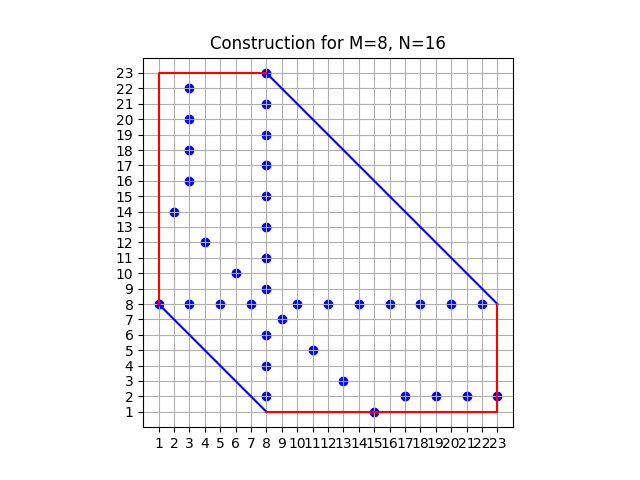
\includegraphics[width=9cm]{round2/p5construct/construct_8_16.png}&
    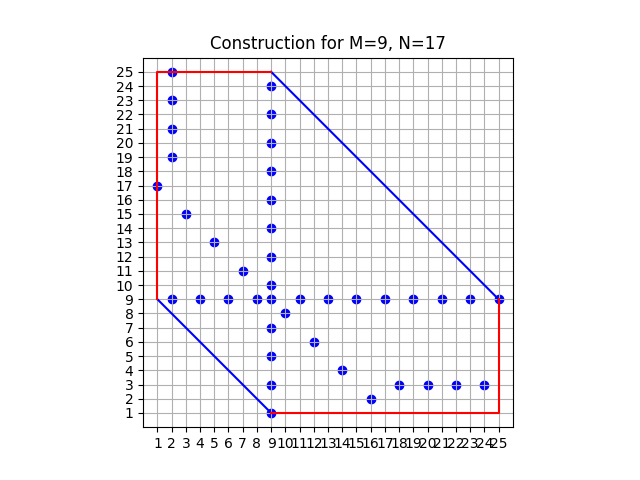
\includegraphics[width=9cm]{round2/p5construct/construct_9_17.png}\\
    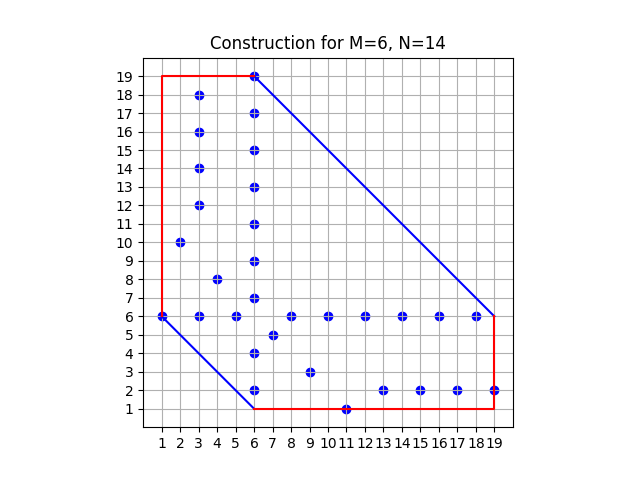
\includegraphics[width=9cm]{round2/p5construct/construct_6_14.png}&
    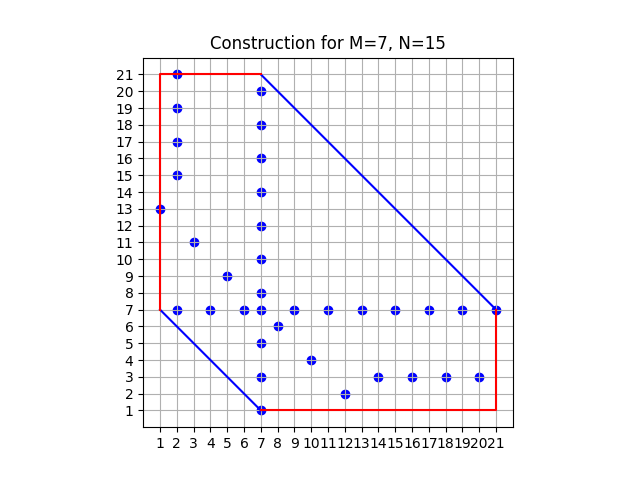
\includegraphics[width=9cm]{round2/p5construct/construct_7_15.png}\\
    \end{tabular}
    \caption{Our construction method applied when m and n are congruent to (going from left to right, top to bottom) 0 mod 4, 1 mod 4, 2 mod 4, 3 mod 4}
    \label{fig:congconstruct}
\end{figure}

\clearpage
We now handle the case where $m \equiv 0 \mod 4$ and $n \equiv 1 \mod 4$ without loss of generality. Again, if the reverse is true, reflect the entire construction across $(m,m)$; this entire problem is translation-independent. We then apply the following steps:

\begin{enumerate}
    \item Select the point $(m,m)$.
    \item \mainaxis
    After this process is done, the lines $x+y = k$ where $m+1 \leq k \leq 2m+n-1$ will each intersect exactly one point from our set.
    \item Select all points of the form $(m-2k, 1+2k)$ for $0 \leq k \leq \floor{\frac{m}{2}}-1$.
    After this process is done, the lines $x=m$, $y=m$, and $x+y = m+1$ will intersect $\floor{\frac{m-1}{2}} + \floor{\frac{n}{2}} + 1 + 1$, $\floor{\frac{n-1}{2}} + \floor{\frac{m}{2}} + 1$, and $\floor{\frac{m}{2}} + 1$ points respectively. Since $m \equiv 0 \mod 4$ and $n \equiv 1 \mod 4$, these expressions are all odd. Furthermore, with the addition of these points, all lines of the form $x=k$ and $y=k$ where $1 \leq k \leq m-1$ will now intersect exactly one point.
    \item Create a ``tail'' to cover all of the outer rows and columns:
    \begin{enumerate}
        \item Select all points of the form $(2, m+2k)$ for $1 \leq k \leq \floor{\frac{n-1}{2}}$
        \item Select all points of the form $(m+2k-1, 3)$ for $1 \leq k \leq \floor{\frac{n-1}{2}}$
    \end{enumerate}
    With the addition of these points, all horizontal and vertical lines now intersect an odd number of points; all lines of the form $x = k$ and $y=k$ for all $m+1 \geq k < m+n$ will intersect exactly one point.
    
    Let the set of points that we selected in Step 4 be denoted $U$. Notice that $\paren{2}+\paren{m+2k} = \paren{m+2k-1}+\paren{3}$. So, every time a line of the form $x+y=c$ for some constant $c$ intersects an element of $U$, it intersects exactly two elements of $U$. So all diagonal lines will continue to intersect an odd number of elements.
\end{enumerate}
Figure \ref{fig:zerooneconstruct} shows how our construction is supposed to appear (consider this to be more authoritative in case of any discrepancies).

\begin{figure}[htbp]
\centering
    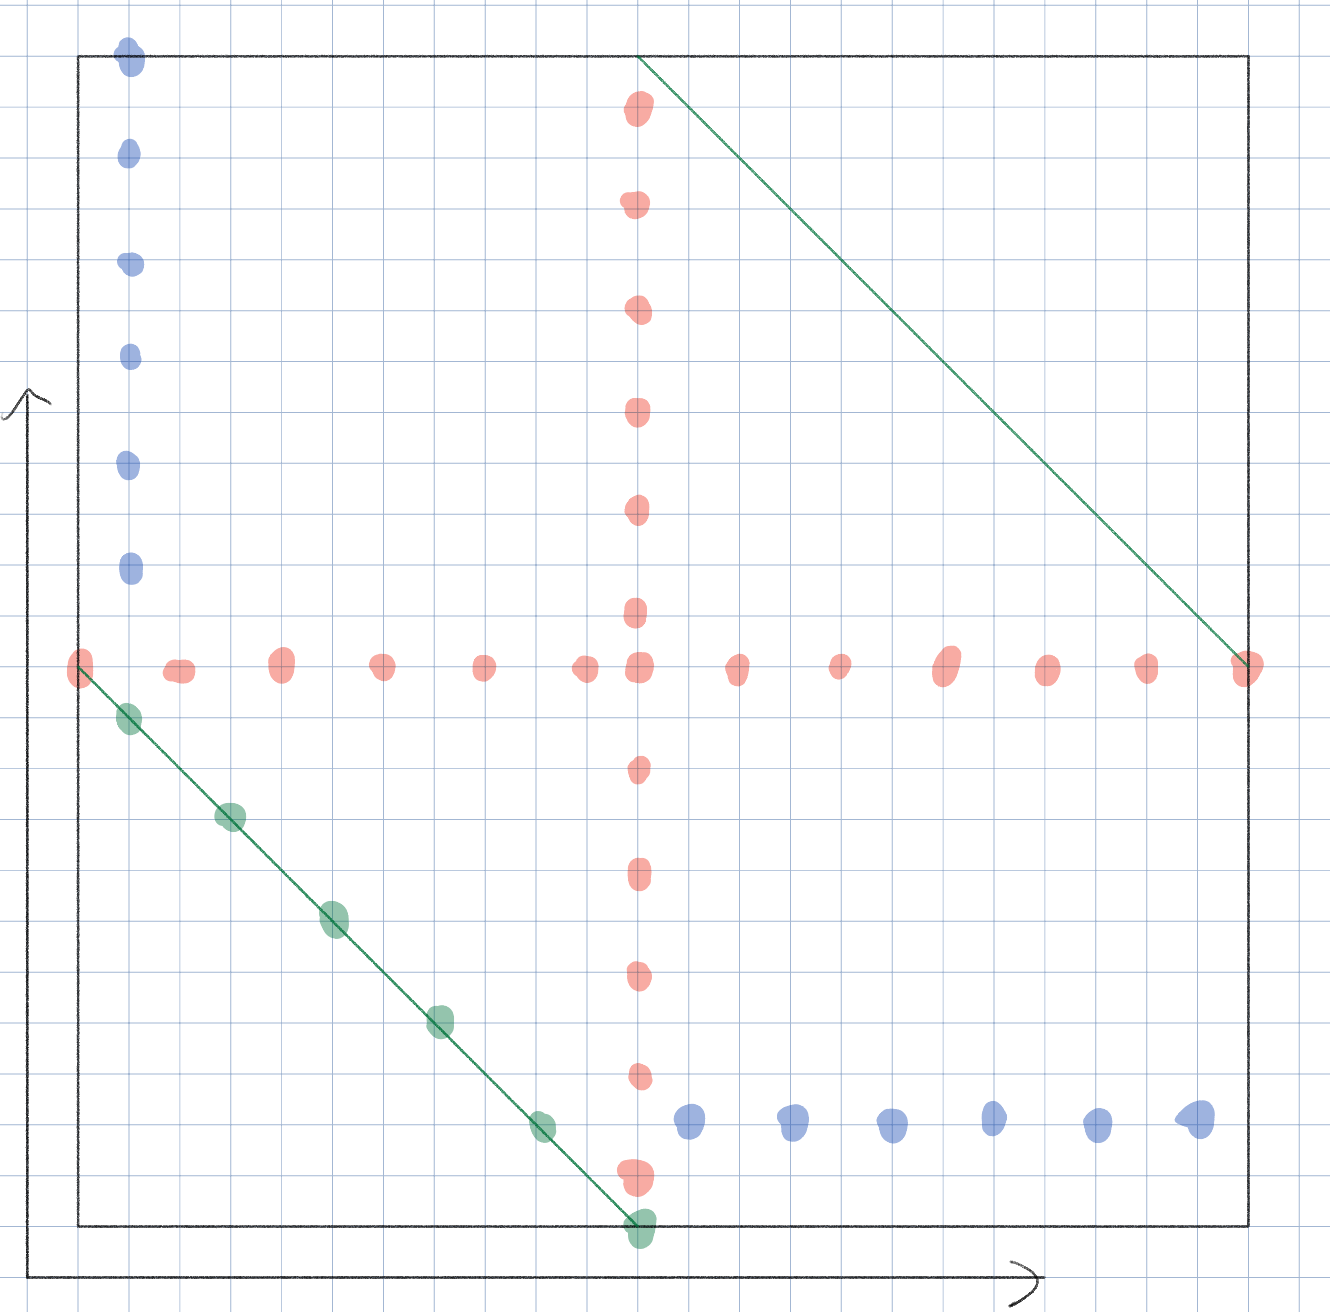
\includegraphics[width=12cm]{round2/p5construct/construct_12_13.png}
    \caption{Construction for when m is congruent to 0 mod 4 and n is congruent to 1 mod 4.}
    \label{fig:zerooneconstruct}
\end{figure}

\clearpage
We now handle the case where $m \equiv 3 \mod 4$ and $n \equiv 2 \mod 4$ without loss of generality (again, if the reverse is true, reflect the entire construction across $(m,m)$). We then apply the following steps:

\begin{enumerate}
    \item Use the construction for when $n=2$
    \begin{enumerate}
        \item Select every point such that $x+y = m+1$.
        \item Select every point on the segment from $\paren{\frac{m+1}{2}, \frac{m+1}{2}}$ to $\paren{\frac{m+1}{2}, m+1}$ inclusive.
        \item Select every point on the segment from $\paren{m+1, \frac{m+1}{2}+1}$ to $\paren{m+1, m}$ inclusive.
    \end{enumerate}
    The line $x+y=m+1$ intersects $m \equiv 1 \mod 2$ points. All other lines of the form $x+y=k$ for $m+1 < k \leq 2m+1$ intersect exactly one point each. The lines $x=\frac{m+1}{2}$ and $x=m+1$ will intersect $\frac{m+3}{2}$ and $\frac{m-1}{2}$ points respectively, which are both odd; all \textbf{other} lines of the form $x=k$ for $0 < k \leq m+1$ intersect exactly one point, which itself will be on the diagonal of $x+y=m+1$. The lines $y=m+1$ and $y=k$ for $1 \leq k \leq \frac{m-1}{2}$ intersect exactly one point, while the lines $y=k$ for $\frac{m+3}{2} \leq k \leq m$ will intersect three points.
    \item Extend the construction to hit all the diagonals.
    \begin{enumerate}
        \item Select every point of the form $(m+1, m+2k)$ for $1 \leq k \leq \frac{n-2}{2}$.
        \item Select every point of the form $(m+2k, m)$ for $1 \leq k \leq \frac{n-2}{2}$.
    \end{enumerate}
    Note that this process allows us to select exactly one point from each diagonal of the form $x+y=k$ where $2m+2 \leq k \leq 2m+n-1$.
    Furthermore, the lines $x=m+1$ and $y=m$ will each intersect $\frac{n-2}{2}$ extra points, which is even.
    \item Complete the construction for all the new rows and columns.
    \begin{enumerate}
        \item Select every point of the form $(1, m+1+2k)$ for $1 \leq k \leq \frac{n-2}{2}$.
        \item Select every point of the form $(m+1+2k, 1)$ for $1 \leq k \leq \frac{n-2}{2}$.
    \end{enumerate}
    After adding these points, every line of the form $x=k$ and $y=k$ where $m+3 \leq k \leq m+n-1$ will intersect exactly one point in our set.
    
    For purposes of notation, let the set of points that we just selected in step 3 be denoted $U$. Notice that $\paren{1}+\paren{m+1+2k} = \paren{m+1+2k}+\paren{1}$. So, every time a line of the form $x+y=c$ for some constant $c$ intersects an element of $U$, it intersects exactly two elements of $U$. So all diagonal lines will continue to intersect an odd number of elements.
\end{enumerate}

Figure \ref{fig:twothreeconstruct} shows how our construction is supposed to appear (consider this to be more authoritative in case of any discrepancies).
\begin{figure}[htbp]
\centering
    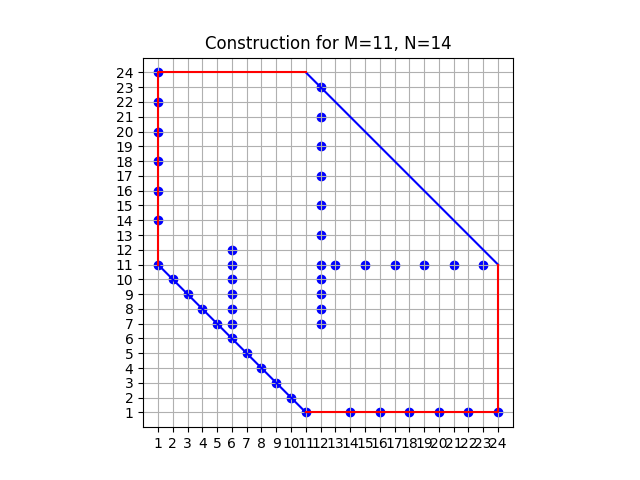
\includegraphics[width=12cm]{round2/p5construct/construct_11_14.png}
    \caption{Construction for when m is congruent to 3 mod 4 and n is congruent to 2 mod 4.}
    \label{fig:twothreeconstruct}
\end{figure}

\clearpage

We also handle a special case where $n \equiv m \mod 4$ but in which $n=1$ or $m=1$. Without loss of generality, let $n=1$ (if the other case is true, just reflect the entire construction afterward).

\begin{enumerate}
    \item Select every point of the form $(k,m+1-k)$ for $1 \le k \le m$. Thus, the diagonal $x+y=m+1$ intersects an odd number of points. Furthermore, every horizontal and vertical line will intersect exactly one point from our set.
    \item Select every point of the form $\paren{\frac{m+1}{2}, \frac{m+1}{2}+k}$ and $\paren{m, \frac{m+1}{2}+k}$ for $1 \le k \le \floor{\frac{m}{2}}$. Now, every horizontal line between $y=\frac{m+1}{2}$ and $y=m$ inclusive intersects exactly three points, and the vertical lines $X=\frac{m+1}{2}$ and $x=m$ both intersect an odd number of points. Furthermore, the other diagonals (other than $x+y=m+1$) now intersect exactly one point, so we are done.
\end{enumerate}

The construction is also visualized in Figure \ref{fig:131construct}.

\begin{figure}[ht]
\centering
    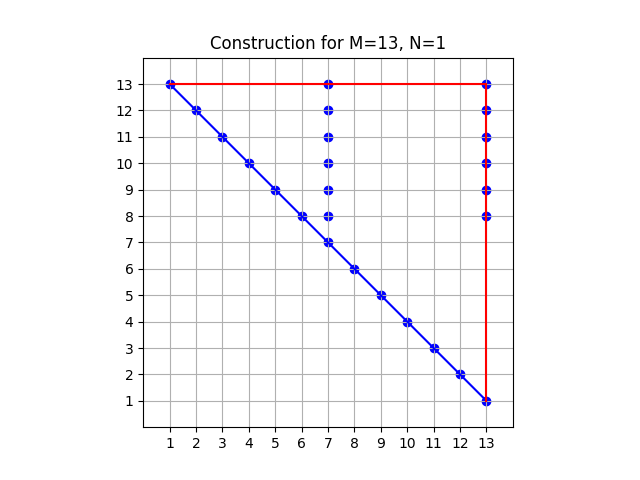
\includegraphics[width=12cm]{round2/p5construct/construct_13_1.png}
    \caption{Construction for $m=13$, $n=1$}
    \label{fig:131construct}
\end{figure}

I also wrote a Python script to automate constructions (and check their correctness) with the source code listed below. Numpy and Matplotlib are required to run it.

\clearpage

\inputminted{python}{p5construct/algorithm.py}

\end{solution}

\end{document}